\chapter{System Design and Architecture}\thispagestyle{thesisstyle} %chapter head
\graphicspath{{Chapter4/figures/}}
{\setstretch{1.5}
%--------------------------------------------------------------------------------------

\section{System Architecture}
Figure~\ref{fig:arch} shows the architecture. Each channel (email, SMS, call audio) has two layers that look at the message itself: a \emph{content model} that reads the text, and a \emph{link or audio layer} that checks the web links or the voice. The three channels then share one \emph{behaviour engine}, which keeps a profile for every sender and caller, and one \emph{fusion} step, which produces the verdict.

\begin{figure}[H]
\centering
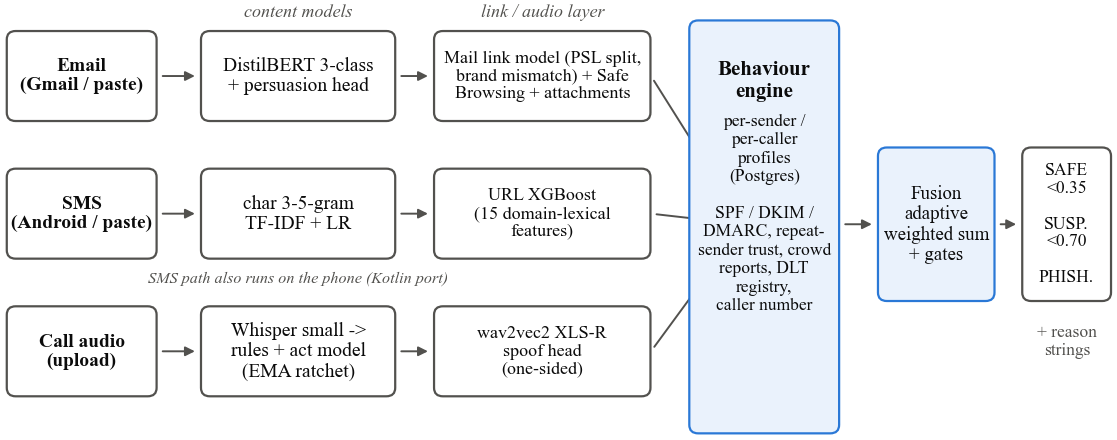
\includegraphics[width=\textwidth]{Chapter4/figures/arch.png}
\caption{System architecture. A channel with no output abstains and its weight is shared among the others. The SMS path also runs on the Android phone.}
\label{fig:arch}
\end{figure}

The path of a message through the system is:
\begin{enumerate}
\item \textbf{Ingest.} The message enters by paste on the website, by the Gmail poller, by the Android SMS receiver, or as an uploaded call recording.
\item \textbf{Preprocess.} Text is normalised (Unicode forms, zero-width characters and look-alike letters are folded), mail headers are read, links are extracted by one shared extractor, and call audio is turned into text by Whisper.
\item \textbf{Models.} The content model scores the text. The link model and Google Safe Browsing score every link. For calls, a synthetic-voice detector scores the audio.
\item \textbf{Behaviour.} The sender's or caller's profile is read from the database and a deviation score is computed. The profile is updated \emph{after} scoring.
\item \textbf{Fusion.} The available scores are combined by a weighted sum, and two safety rules are applied. The risk is mapped to Safe (below 0.35), Suspicious (0.35 to 0.70) or Phishing (0.70 and above).
\item \textbf{Output.} The verdict and the list of reasons are returned and stored, and shown to the user.
\end{enumerate}

\section{Hardware Architecture}
The project has no special hardware. All of it runs on ordinary computing devices. The development laptop hosts the PostgreSQL database, the model service and the dashboard. The user's browser reaches the dashboard, the dashboard reaches the model service on the same machine, and the Android phone runs its own copy of the SMS models and needs no connection to any of them. Table~\ref{tab:hw} in Chapter~3 lists the machine used.

\section{Software Module Design}
\subsection{Model service modules}
Table~\ref{tab:modpy} lists the Python modules.

\begin{table}[H]
\caption{Python model service modules}
\label{tab:modpy}
\centering\small\setstretch{1.05}
\begin{tabular}{|p{3.6cm}|p{10.6cm}|}
\hline
\textbf{Module} & \textbf{Role} \\ \hline
\texttt{api.py} & FastAPI service that exposes the endpoints and ties the models, behaviour engine and fusion together \\ \hline
\texttt{data.py} & Dataset loaders (all labels mapped so that 1 means malicious), mail parsing, link-host extraction \\ \hline
\texttt{sms\_model.py} & SMS model: character 3--5-gram TF-IDF with logistic regression, three classes (ham, spam, smishing) \\ \hline
\texttt{email\_model.py} & Email model: DistilBERT with three classes and a second head for five persuasion principles \\ \hline
\texttt{url\_model.py} & Link model: XGBoost on domain-only features, with a mail variant that uses the Public Suffix List and brand-mismatch checks \\ \hline
\texttt{attachments.py} & Dangerous file types and links found inside PDF, HTML, SVG and calendar attachments \\ \hline
\texttt{safe\_browsing.py} & Google Safe Browsing v5 lookup using hash prefixes only \\ \hline
\texttt{voice\_model.py} & Speech risk: rule patterns, an asymmetric moving average, and the call verdict \\ \hline
\texttt{act\_model.py}, \texttt{llm\_primitives.py} & DistilBERT model that spots scam moves in a call, trained on labels from a larger language model \\ \hline
\texttt{spoof\_model.py} & Synthetic-voice detector: frozen wav2vec2 XLS-R features with a logistic-regression head \\ \hline
\texttt{behaviour.py} & Sender and caller profiles, deviation features, SPF/DKIM/DMARC check, SMS header registry check, caller-number rules \\ \hline
\texttt{fusion.py} & Adaptive weighted sum, the escalation and uncertainty rules, and the band mapping \\ \hline
\texttt{thread.py} & Rolling score over a series of SMS from one sender \\ \hline
\texttt{adversarial.py} & Unicode normalisation and obfuscation used to augment the training data \\ \hline
\texttt{store.py} & PostgreSQL persistence for sender profiles, feedback and crowd reports \\ \hline
\texttt{export\_android.py} & Exports the SMS and link models for the phone and writes the parity test files \\ \hline
\end{tabular}
\end{table}

\subsection{Model service endpoints}
Table~\ref{tab:api} lists the endpoints of the model service.

\begin{table}[H]
\caption{Endpoints of the model service}
\label{tab:api}
\centering\small\setstretch{1.05}
\begin{tabular}{|p{3.4cm}|p{10.8cm}|}
\hline
\textbf{Endpoint} & \textbf{Purpose} \\ \hline
\texttt{POST /sms} & Score one SMS, with an optional sender header \\ \hline
\texttt{POST /email} & Score an email pasted as text \\ \hline
\texttt{POST /email/raw} & Score a full raw message with headers (used for Gmail), including authentication results and attachments \\ \hline
\texttt{POST /email/parse} & Parse a raw message for display only; it does not score the message or change any profile \\ \hline
\texttt{POST /email/seed} & On Gmail connection, fold the headers of recent mail into the sender profiles without scoring anything \\ \hline
\texttt{POST /email/forget} & On Gmail disconnection, drop the cached profile store of that user \\ \hline
\texttt{POST /voice/text} & Score a call transcript, with an optional caller number \\ \hline
\texttt{POST /voice/file} & Transcribe and score uploaded call audio, including the synthetic-voice check \\ \hline
\texttt{GET /health} & Report that the service is running \\ \hline
\end{tabular}
\end{table}

\subsection{Web dashboard}
The dashboard is built with Next.js 16 and React 19. The page and route structure is:
\begin{itemize}
\item \textbf{Pages:} sign-in and sign-up; a dashboard page with history and a risk timeline; separate pages for email, SMS and voice; a Gmail page; and a phone page that offers the APK for download.
\item \textbf{API routes:} \texttt{scan}, \texttt{scans}, \texttt{voice}, \texttt{ocr}, \texttt{feedback} and \texttt{gmail}. All of them check the session first and forward model work to the model service.
\item \textbf{Libraries:} \texttt{db.js} holds the whole schema and every query, \texttt{auth.js} and \texttt{hash.js} handle sessions and passwords, and \texttt{gmail.js} polls Gmail. The poller is started once, when the server starts, and runs every 60 seconds.
\item \textbf{Components:} the verdict panel (plain-language explanation plus a ``Technical details'' section), the Gmail card, the risk timeline and the screenshot input.
\end{itemize}

\subsection{Android app}
The app is written in Kotlin and has this flow: \texttt{SmsReceiver} receives each message, \texttt{MessageStore} keeps it in a local Room database, \texttt{Classifier} scores it using \texttt{LocalScan}, which contains Kotlin ports of the SMS model, the link model, the behaviour rules and the fusion rule. \texttt{Audit} scores the whole inbox in one pass, and \texttt{Redact} masks codes, amounts, account numbers and addresses before any report is shared. The app asks only for the permissions to read and receive SMS.

\section{Security and Access Control}\label{sec:sec}
Because the system reads personal messages, security and privacy were designed in from the start.
\begin{itemize}
\item \textbf{Sign-in.} A password must have at least eight characters, one uppercase letter and one number. Passwords are hashed with scrypt and a random 16-byte salt, and compared in constant time. The session is a signed token (HMAC-SHA-256) in an HttpOnly cookie that is valid for one week. Every API route checks the session before doing anything.
\item \textbf{Gmail access.} Only the read-only scope is requested. The refresh token is encrypted with AES-GCM under the server secret before it is stored. If Google stops honouring the token, the page asks the user to reconnect.
\item \textbf{Data minimisation.} Mail bodies are never stored. When the user opens a message, the body is fetched live from Gmail and discarded. A stored scan keeps the verdict, the score, the reasons, a short preview and, for attachments, the file type but never the file name.
\item \textbf{Link checks.} Only the first 4 bytes of the SHA-256 hash of a link are sent to Google Safe Browsing, never the link itself.
\item \textbf{Phone.} The app has no internet permission, so neither messages nor verdicts can leave the phone. Its SMS vocabulary is built from public corpora only, so no private text is shipped inside the app. The only thing that can leave is the audit report, which the user chooses to share and which is masked first.
\item \textbf{Per-user separation.} Scans and profiles are keyed by the user, and ingestion is idempotent, so a message is never filed twice.
\item \textbf{Resistance to manipulation.} A repeat sender is trusted only if its mail passes authentication and every link stays on its own domain. Reports from other users count only if they come from at least three different users whose copy of the mail passed DMARC. A vouch for a sender is ignored when the message failed the DMARC check, and the address is read from the angle brackets so that a forged display name cannot vouch for another address.
\end{itemize}

\section{Database Design}
All persistent data is kept in one PostgreSQL database with three tables (Figure~\ref{fig:er}). The whole schema is a single script that is safe to run again: new columns are added with \texttt{ALTER ... IF NOT EXISTS}, so an existing database upgrades itself.

\begin{figure}[H]
\centering
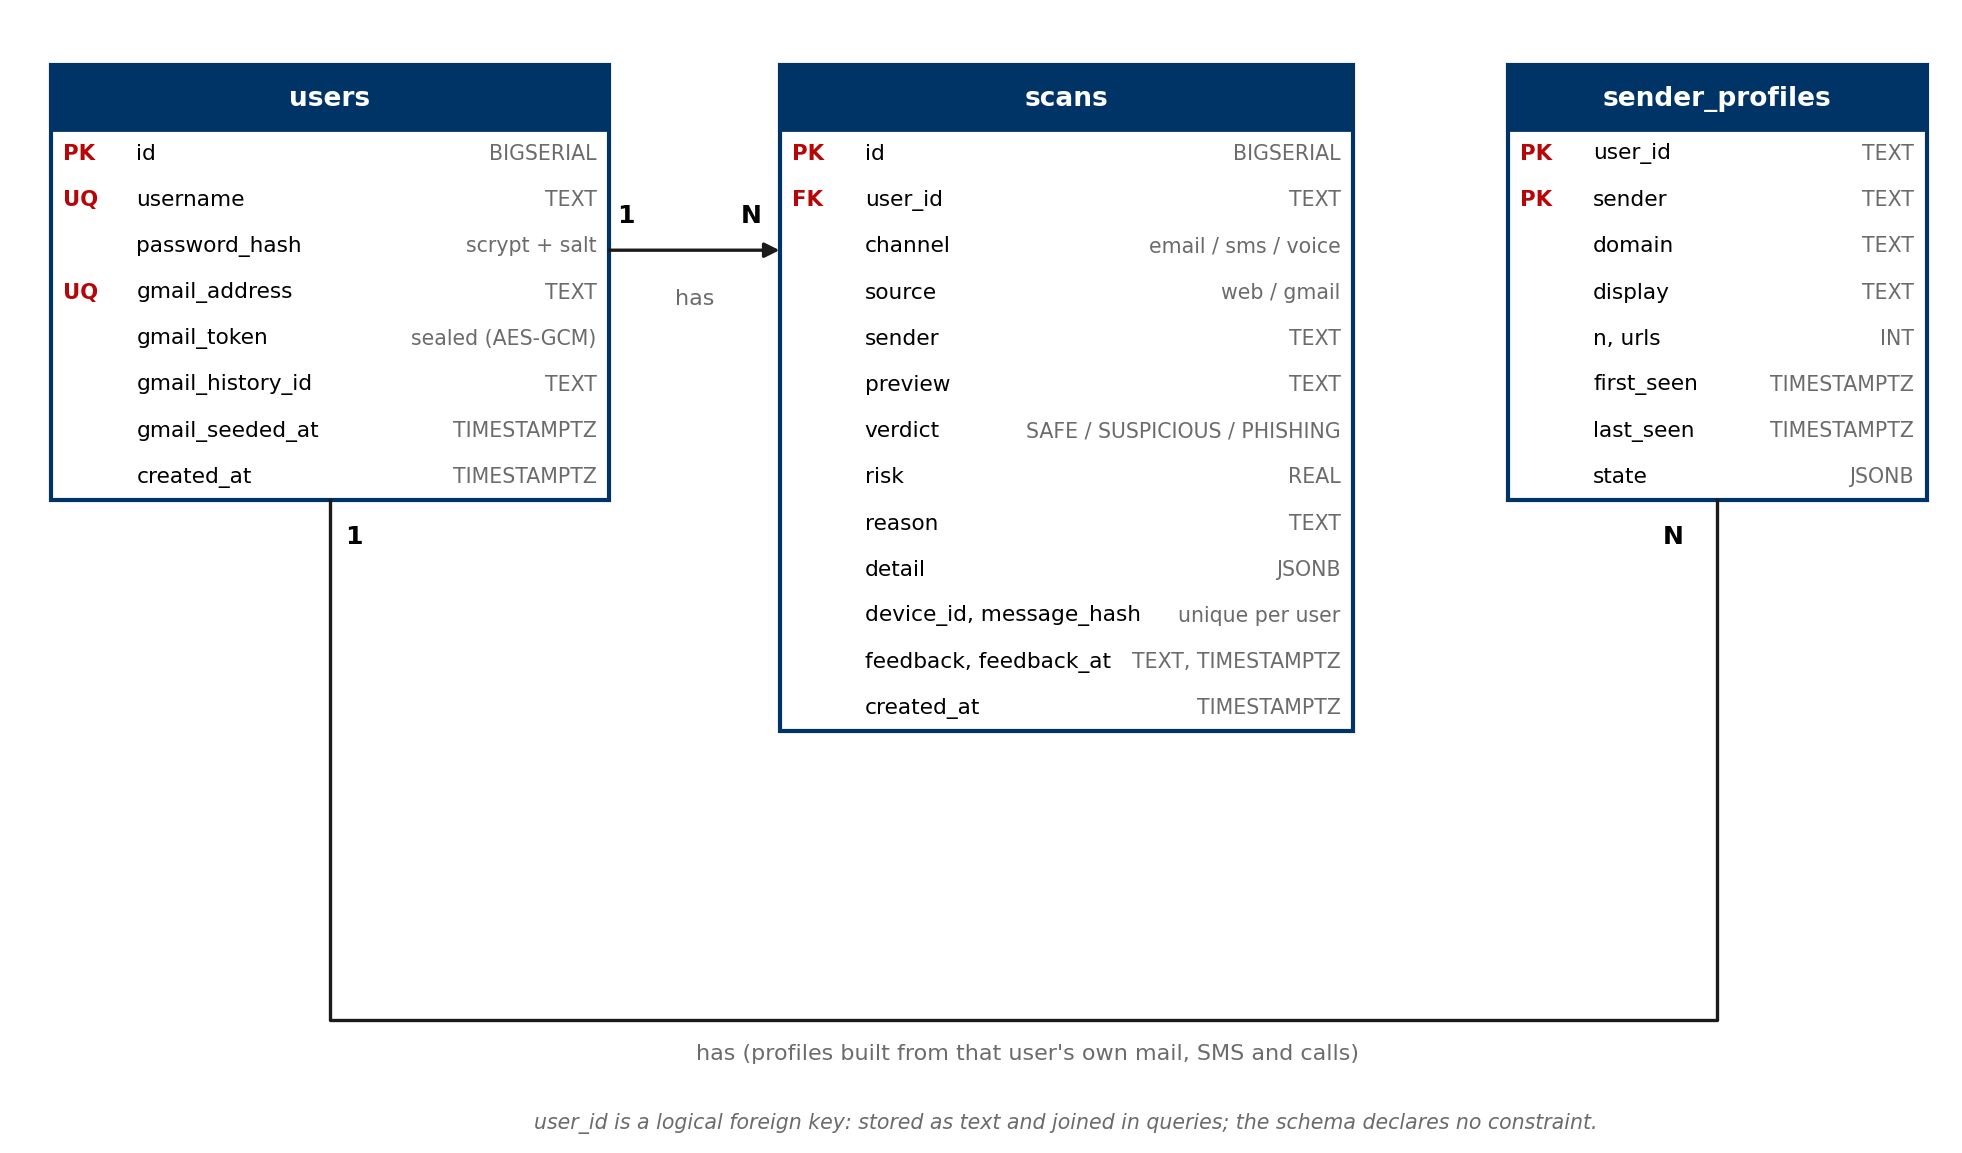
\includegraphics[width=\textwidth]{Chapter4/figures/er.png}
\caption{Entity-relationship diagram of the database}
\label{fig:er}
\end{figure}

\begin{itemize}
\item \textbf{users} holds the login and, in the same row, the Gmail link (address, sealed token and the last history position), because one account has one mailbox.
\item \textbf{scans} holds the history. Its \texttt{source} column says whether the scan came from the website or from Gmail, and \texttt{detail} stores the full result as JSON. A unique index on user, device and message hash makes Gmail ingestion idempotent. The \texttt{feedback} column holds the user's correction.
\item \textbf{sender\_profiles} holds one row per user and sender. It is written only by the Python code, so the model service works whether or not the website was ever started. The \texttt{state} column keeps the activity history used to detect changes in behaviour (usual hours, recipients and writing style).
\end{itemize}

\section{Data Flow Diagrams}
\subsection{Level 0 (context diagram)}
Figure~\ref{fig:dfd0} shows the whole system as one process. The user sends a message, a call or a sender number and receives a verdict with reasons. Gmail supplies new mail, Google Safe Browsing answers link lookups, and Gemini turns a screenshot into text.

\begin{figure}[H]
\centering
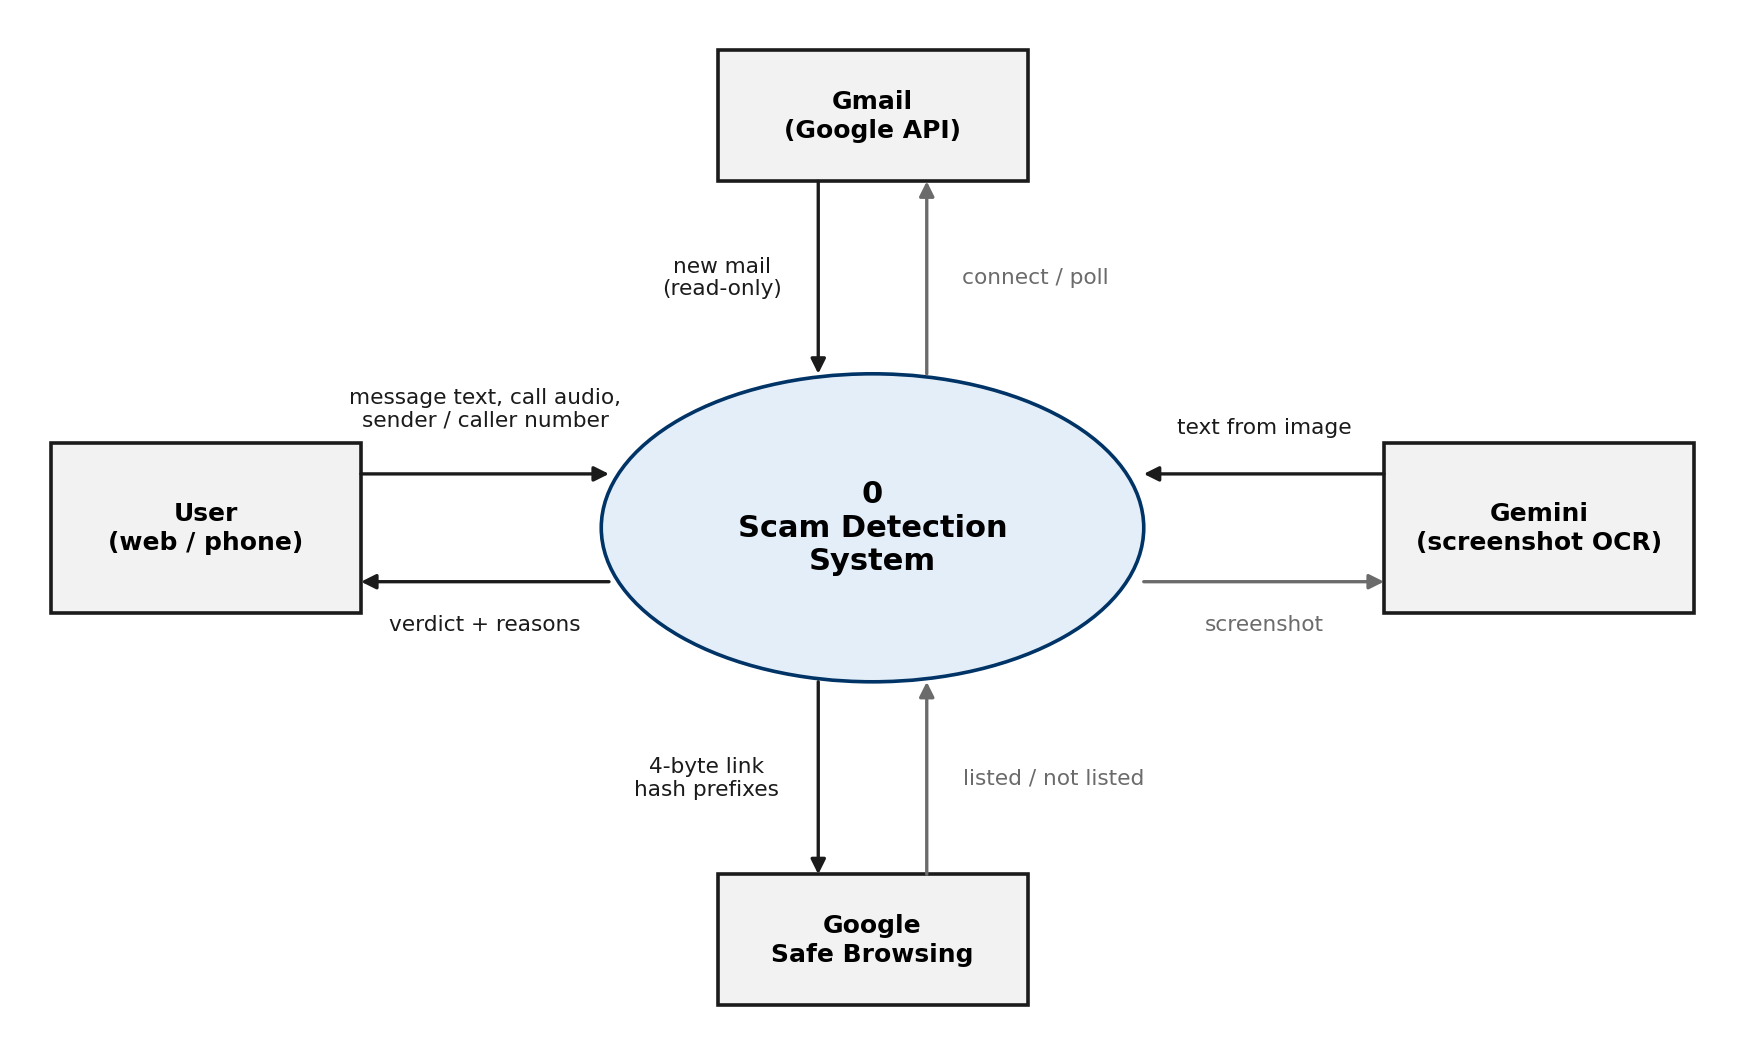
\includegraphics[width=0.92\textwidth]{Chapter4/figures/dfd0.png}
\caption{Data flow diagram, level 0}
\label{fig:dfd0}
\end{figure}

\subsection{Level 1}
Figure~\ref{fig:dfd1} opens the system into six processes. Input is cleaned (1.0) and passed to three scoring processes: content (2.0), links (3.0) and sender behaviour (4.0). The three scores meet in the fusion process (5.0), and the result is saved and shown (6.0). Process 4.0 reads and updates the sender profiles (D2), and process 6.0 writes the scan (D3). Feedback in D3 flows back to behaviour scoring as crowd reports.

\begin{figure}[H]
\centering
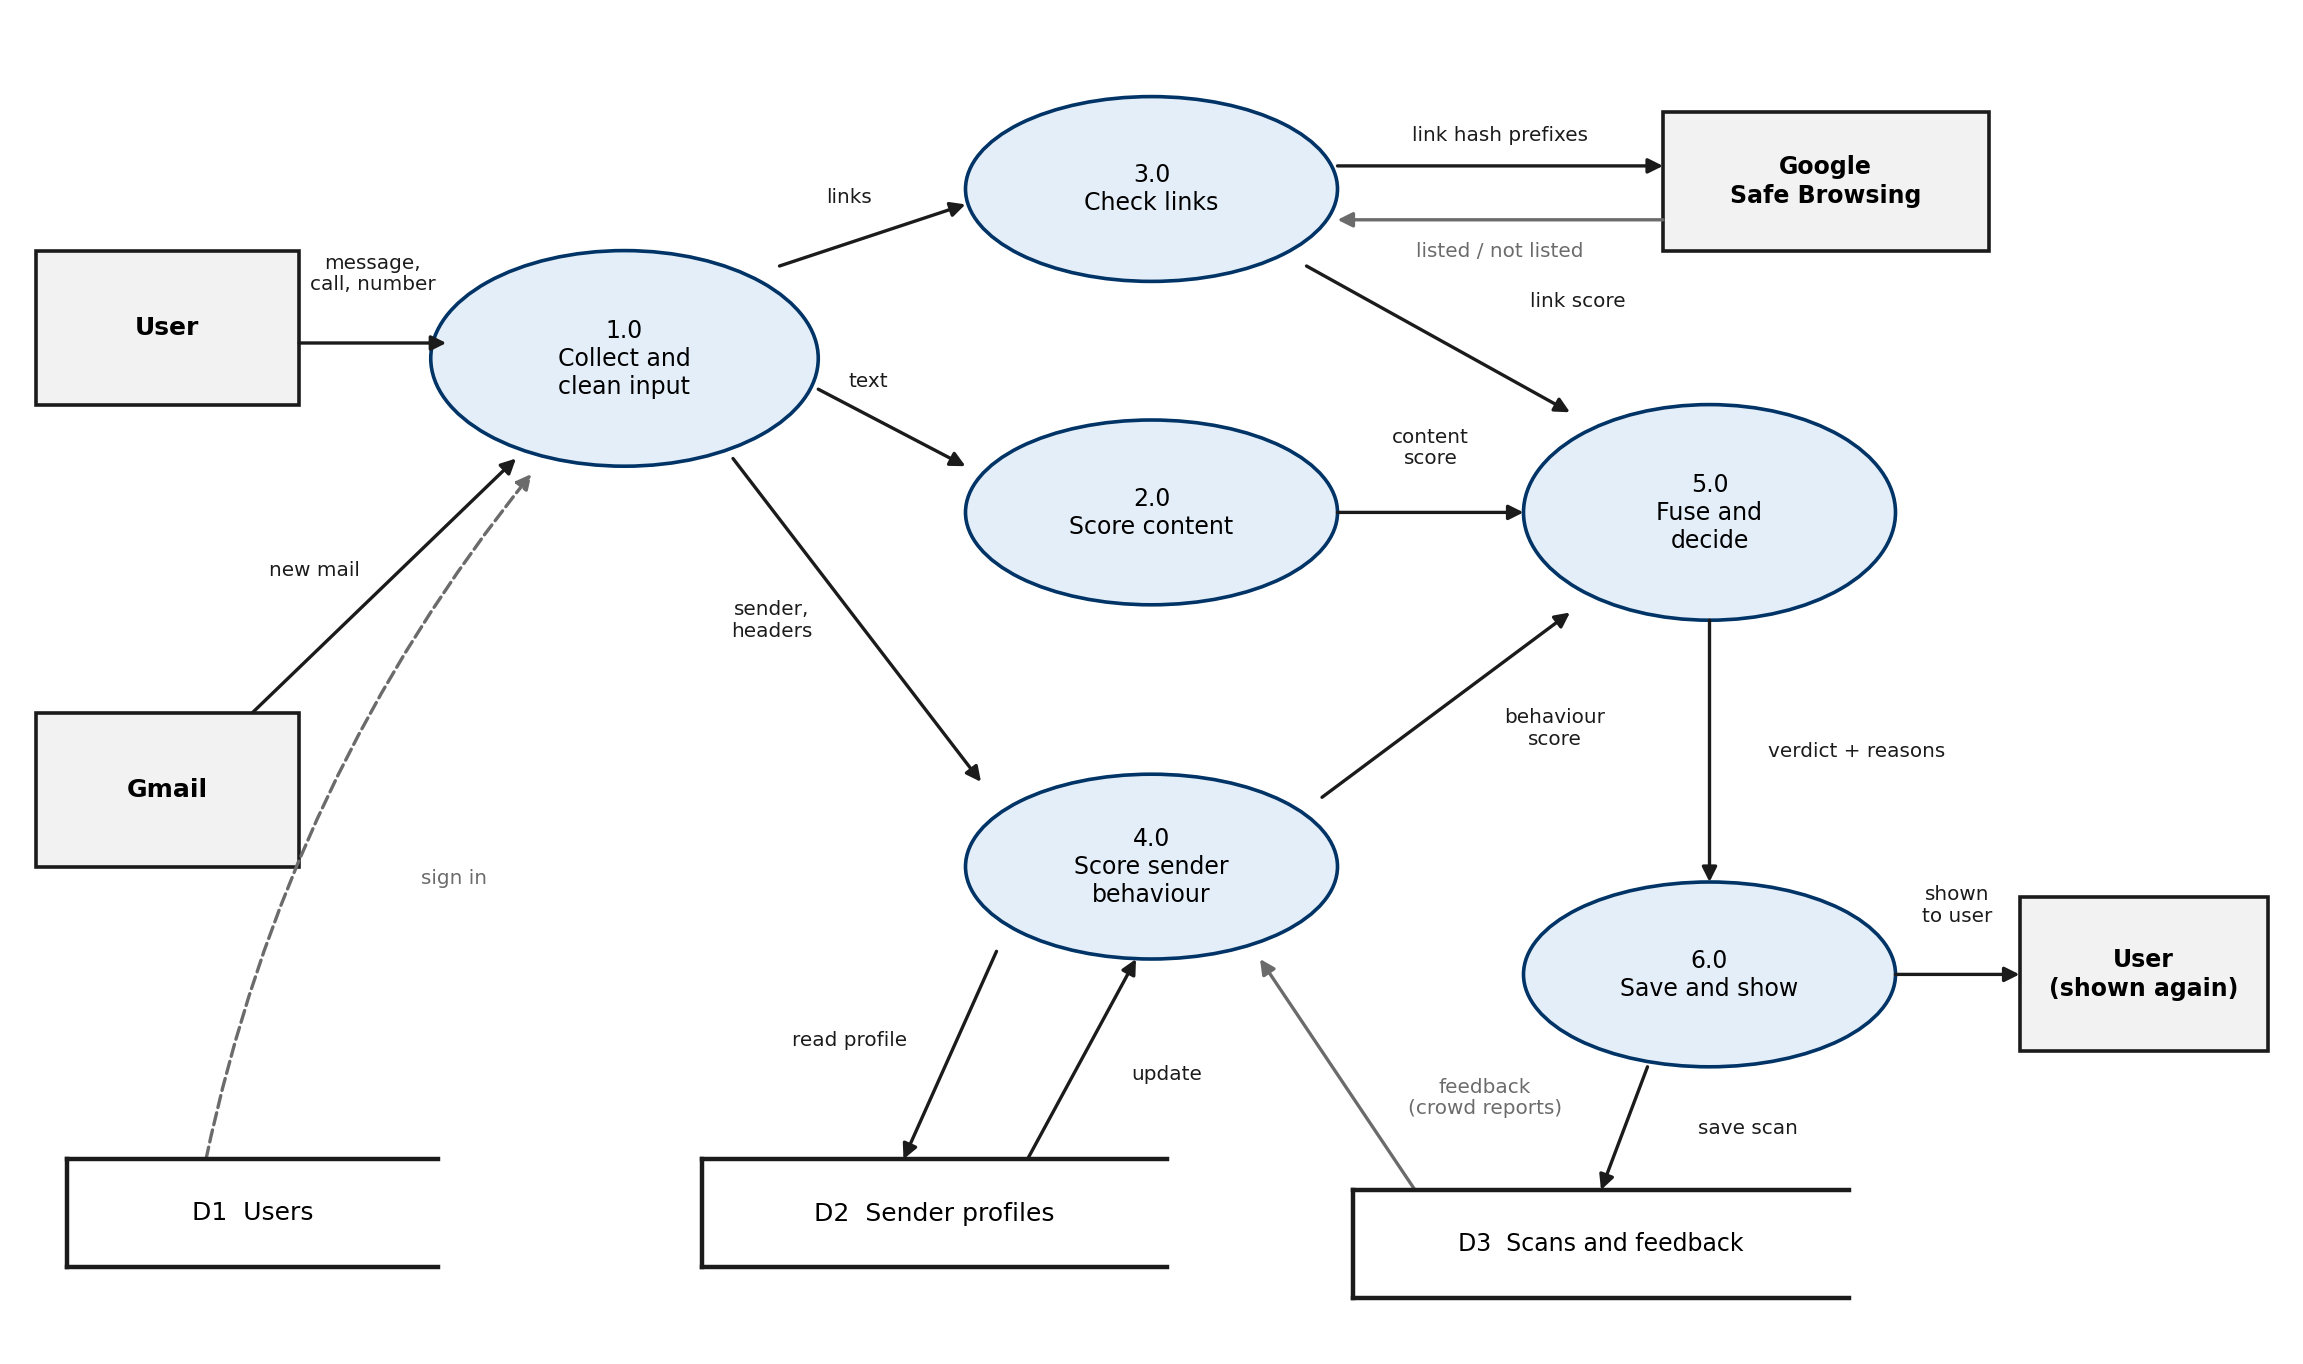
\includegraphics[width=\textwidth]{Chapter4/figures/dfd1.png}
\caption{Data flow diagram, level 1}
\label{fig:dfd1}
\end{figure}

\section{Use Case Diagram}
Figure~\ref{fig:uc} shows the use cases. The web user can sign in, check a pasted email, SMS or call, connect Gmail, view Gmail verdicts, give feedback and view history. The phone user can install the app, get an SMS verdict on the phone and run an inbox audit. Gmail and Google Safe Browsing take part as external actors.

\begin{figure}[H]
\centering
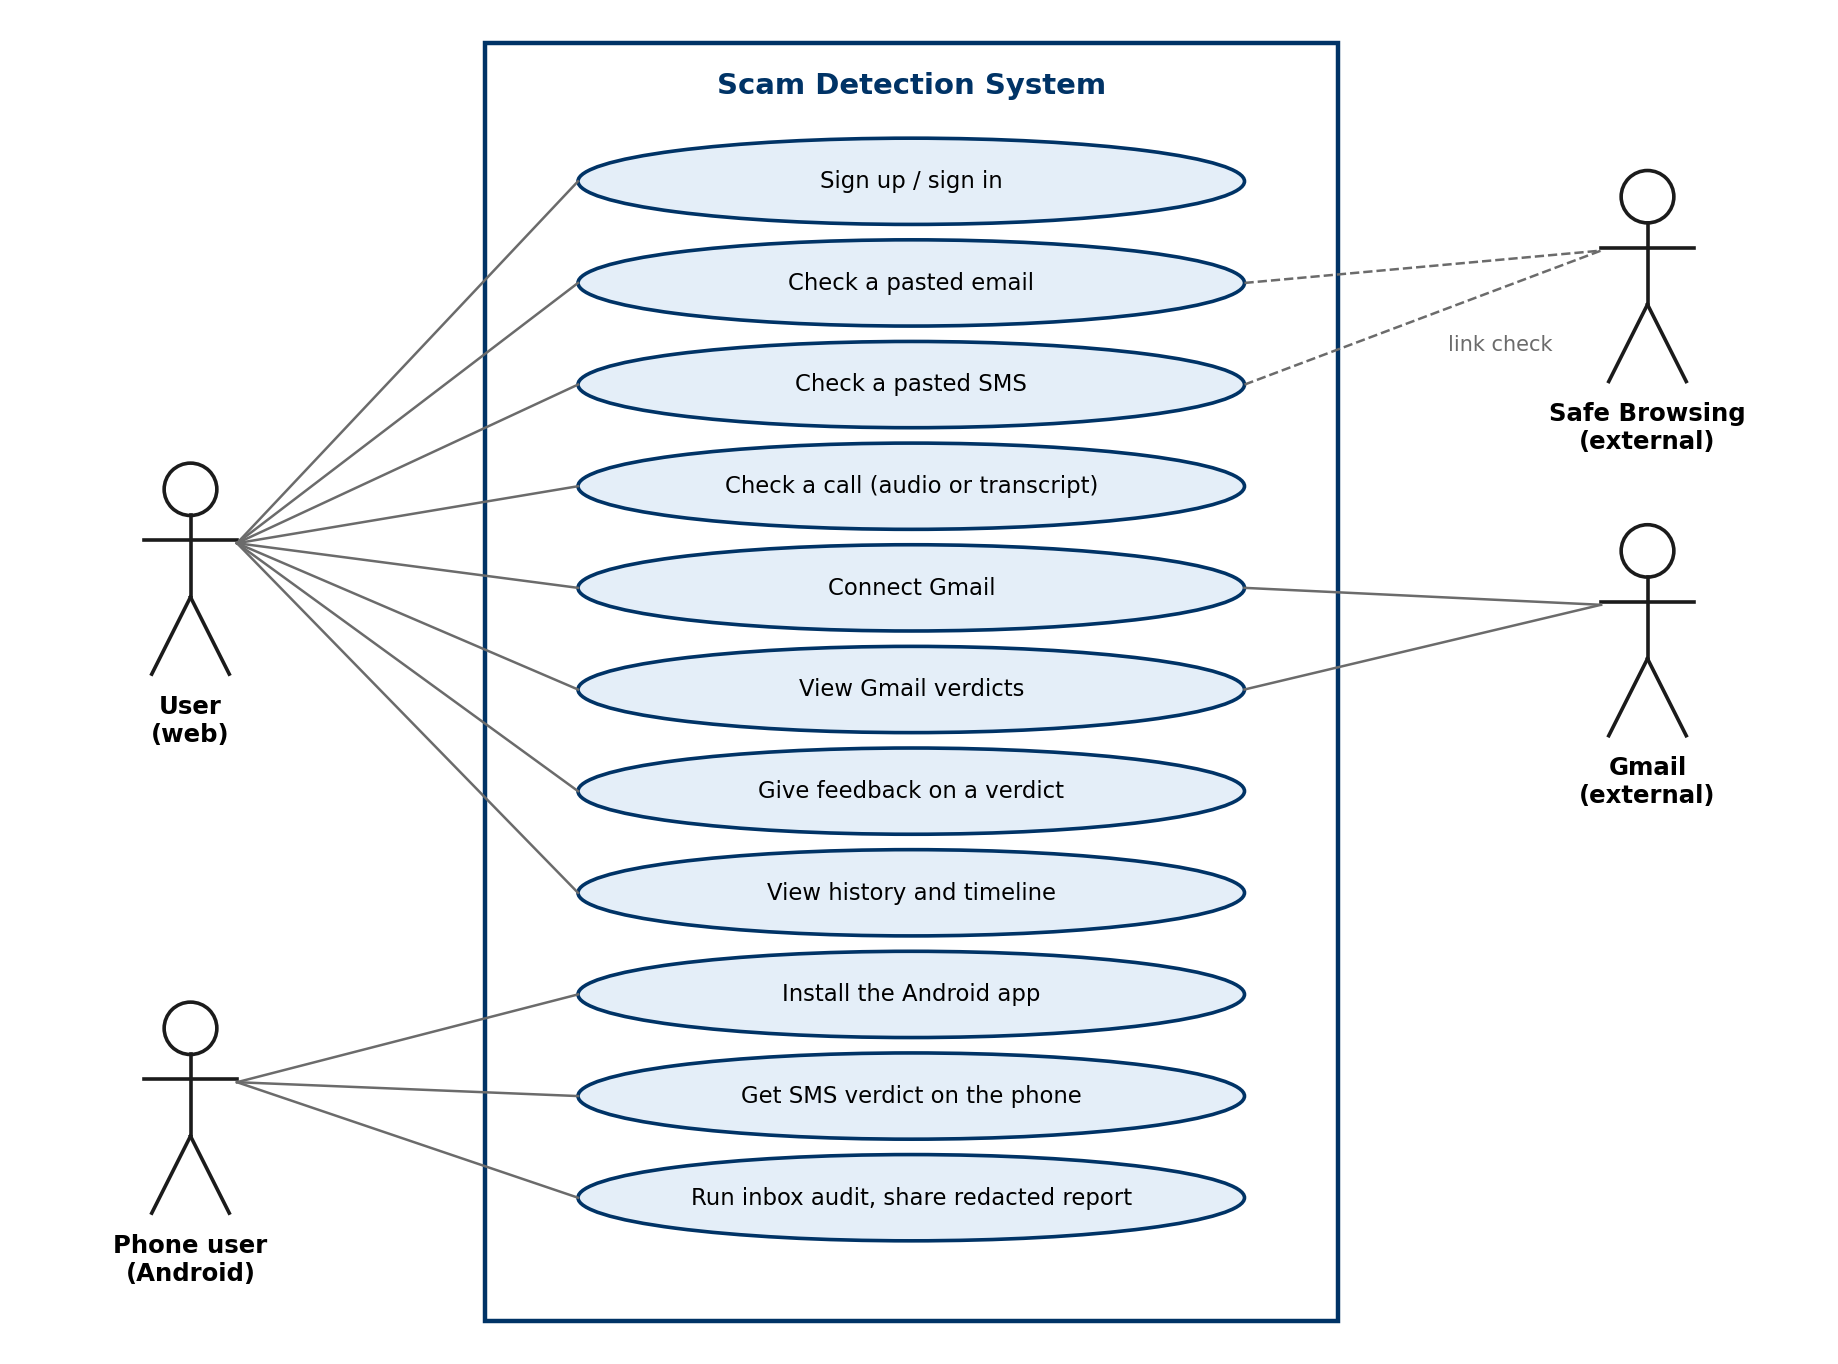
\includegraphics[width=0.9\textwidth]{Chapter4/figures/usecase.png}
\caption{Use case diagram}
\label{fig:uc}
\end{figure}

\section{Activity Diagram}
Figure~\ref{fig:act} follows one message from arrival to verdict. The two decisions show how the system abstains: with no link there is no link score, and with too few known senders there is no behaviour score. In both cases the other scores are used and the weights are shared out among them.

\begin{figure}[H]
\centering
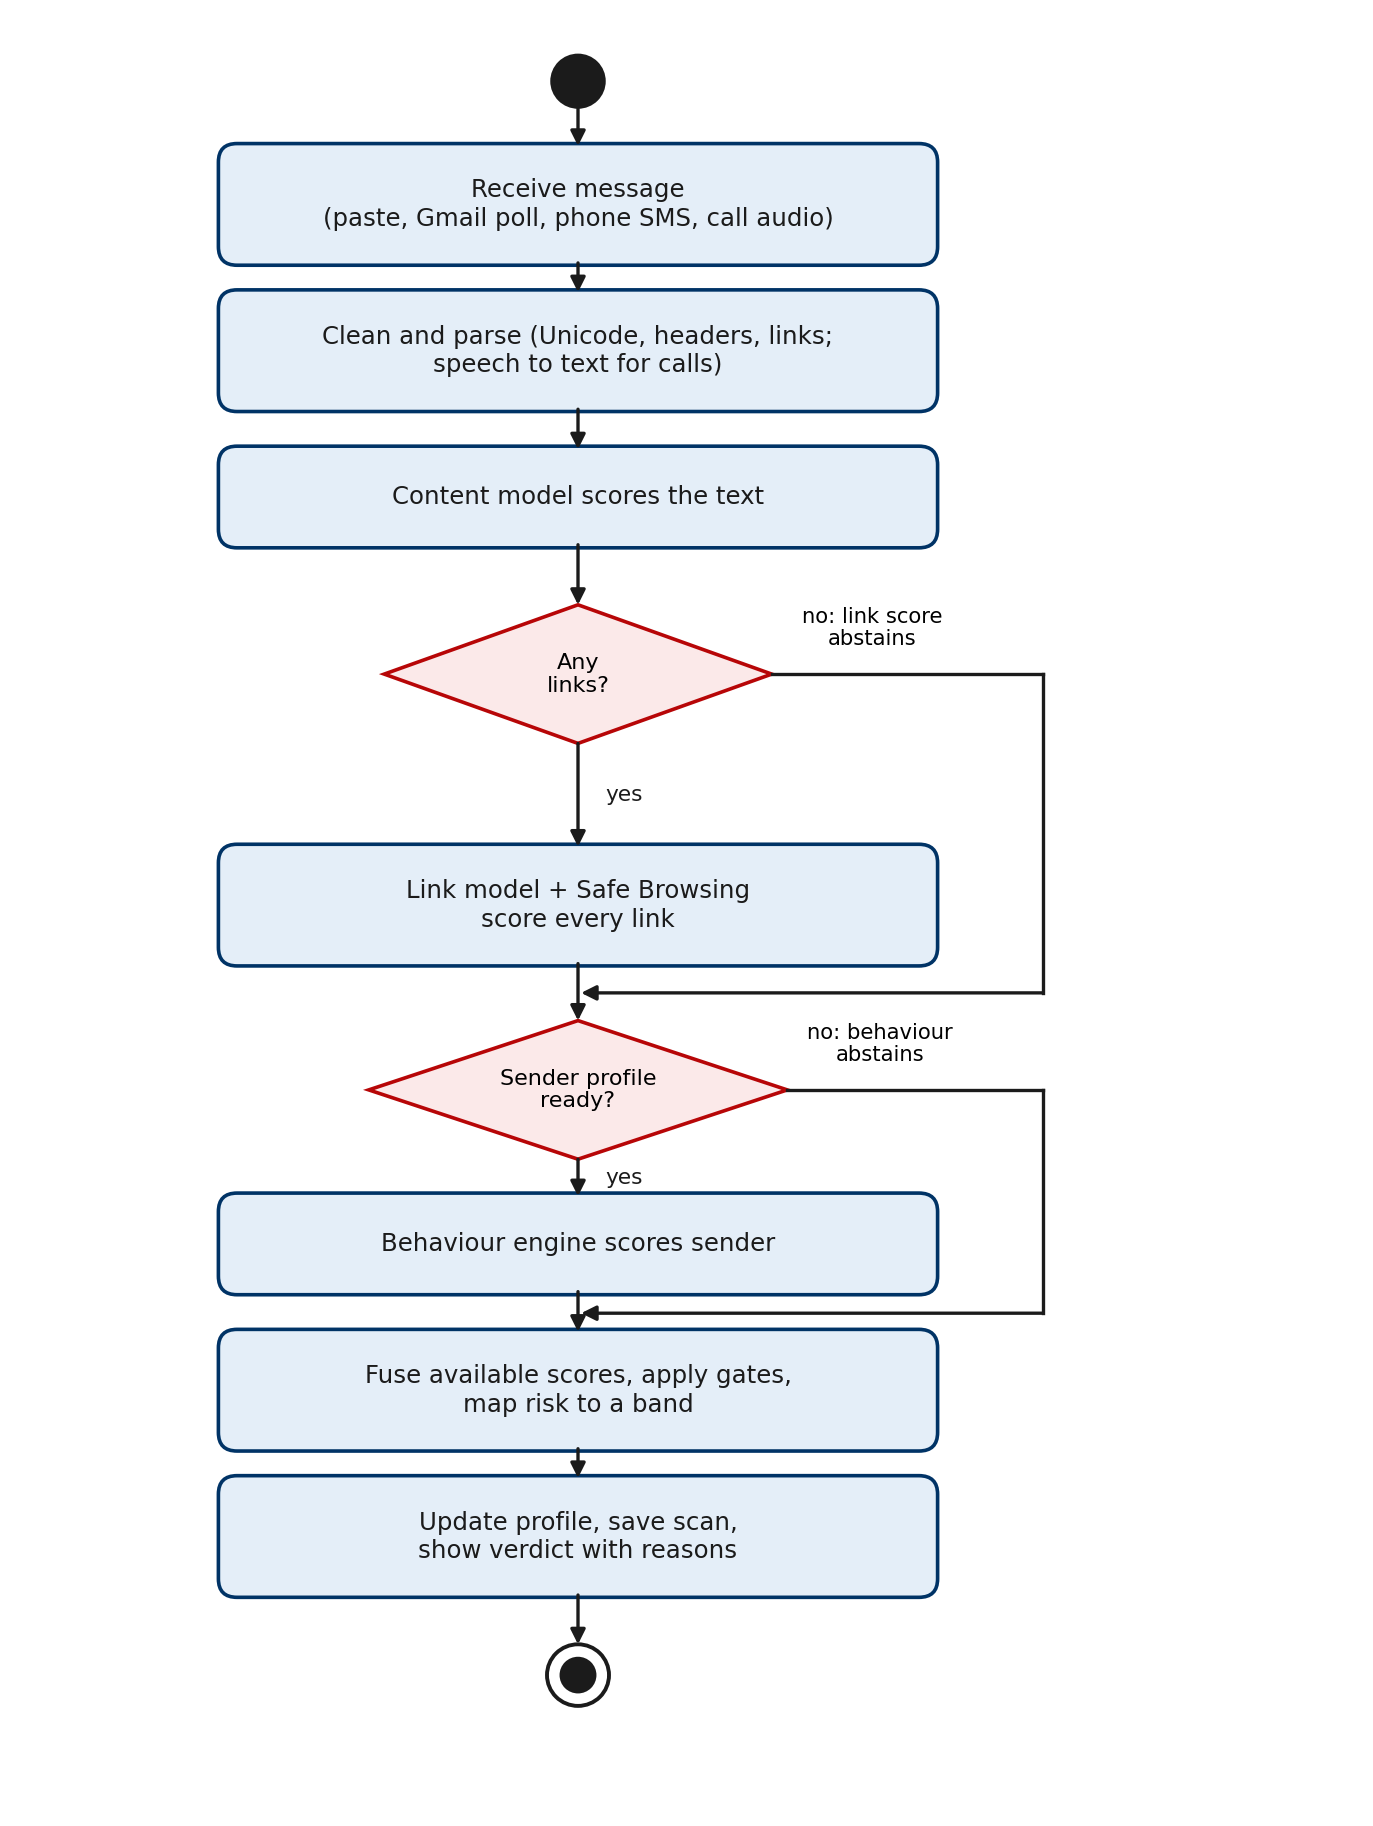
\includegraphics[height=0.62\textheight]{Chapter4/figures/activity.png}
\caption{Activity diagram for checking one message}
\label{fig:act}
\end{figure}

\section{Sequence Diagram}
Figure~\ref{fig:seq} shows how one Gmail message is checked. The dashboard asks Gmail for new mail every 60 seconds and sends each new message to the model service. The model service runs the content and link models, asks Safe Browsing about the links, reads the sender profile, fuses the scores, updates the profile and returns the verdict. The dashboard then saves the scan, without the mail body, and shows the verdict.

\begin{figure}[H]
\centering
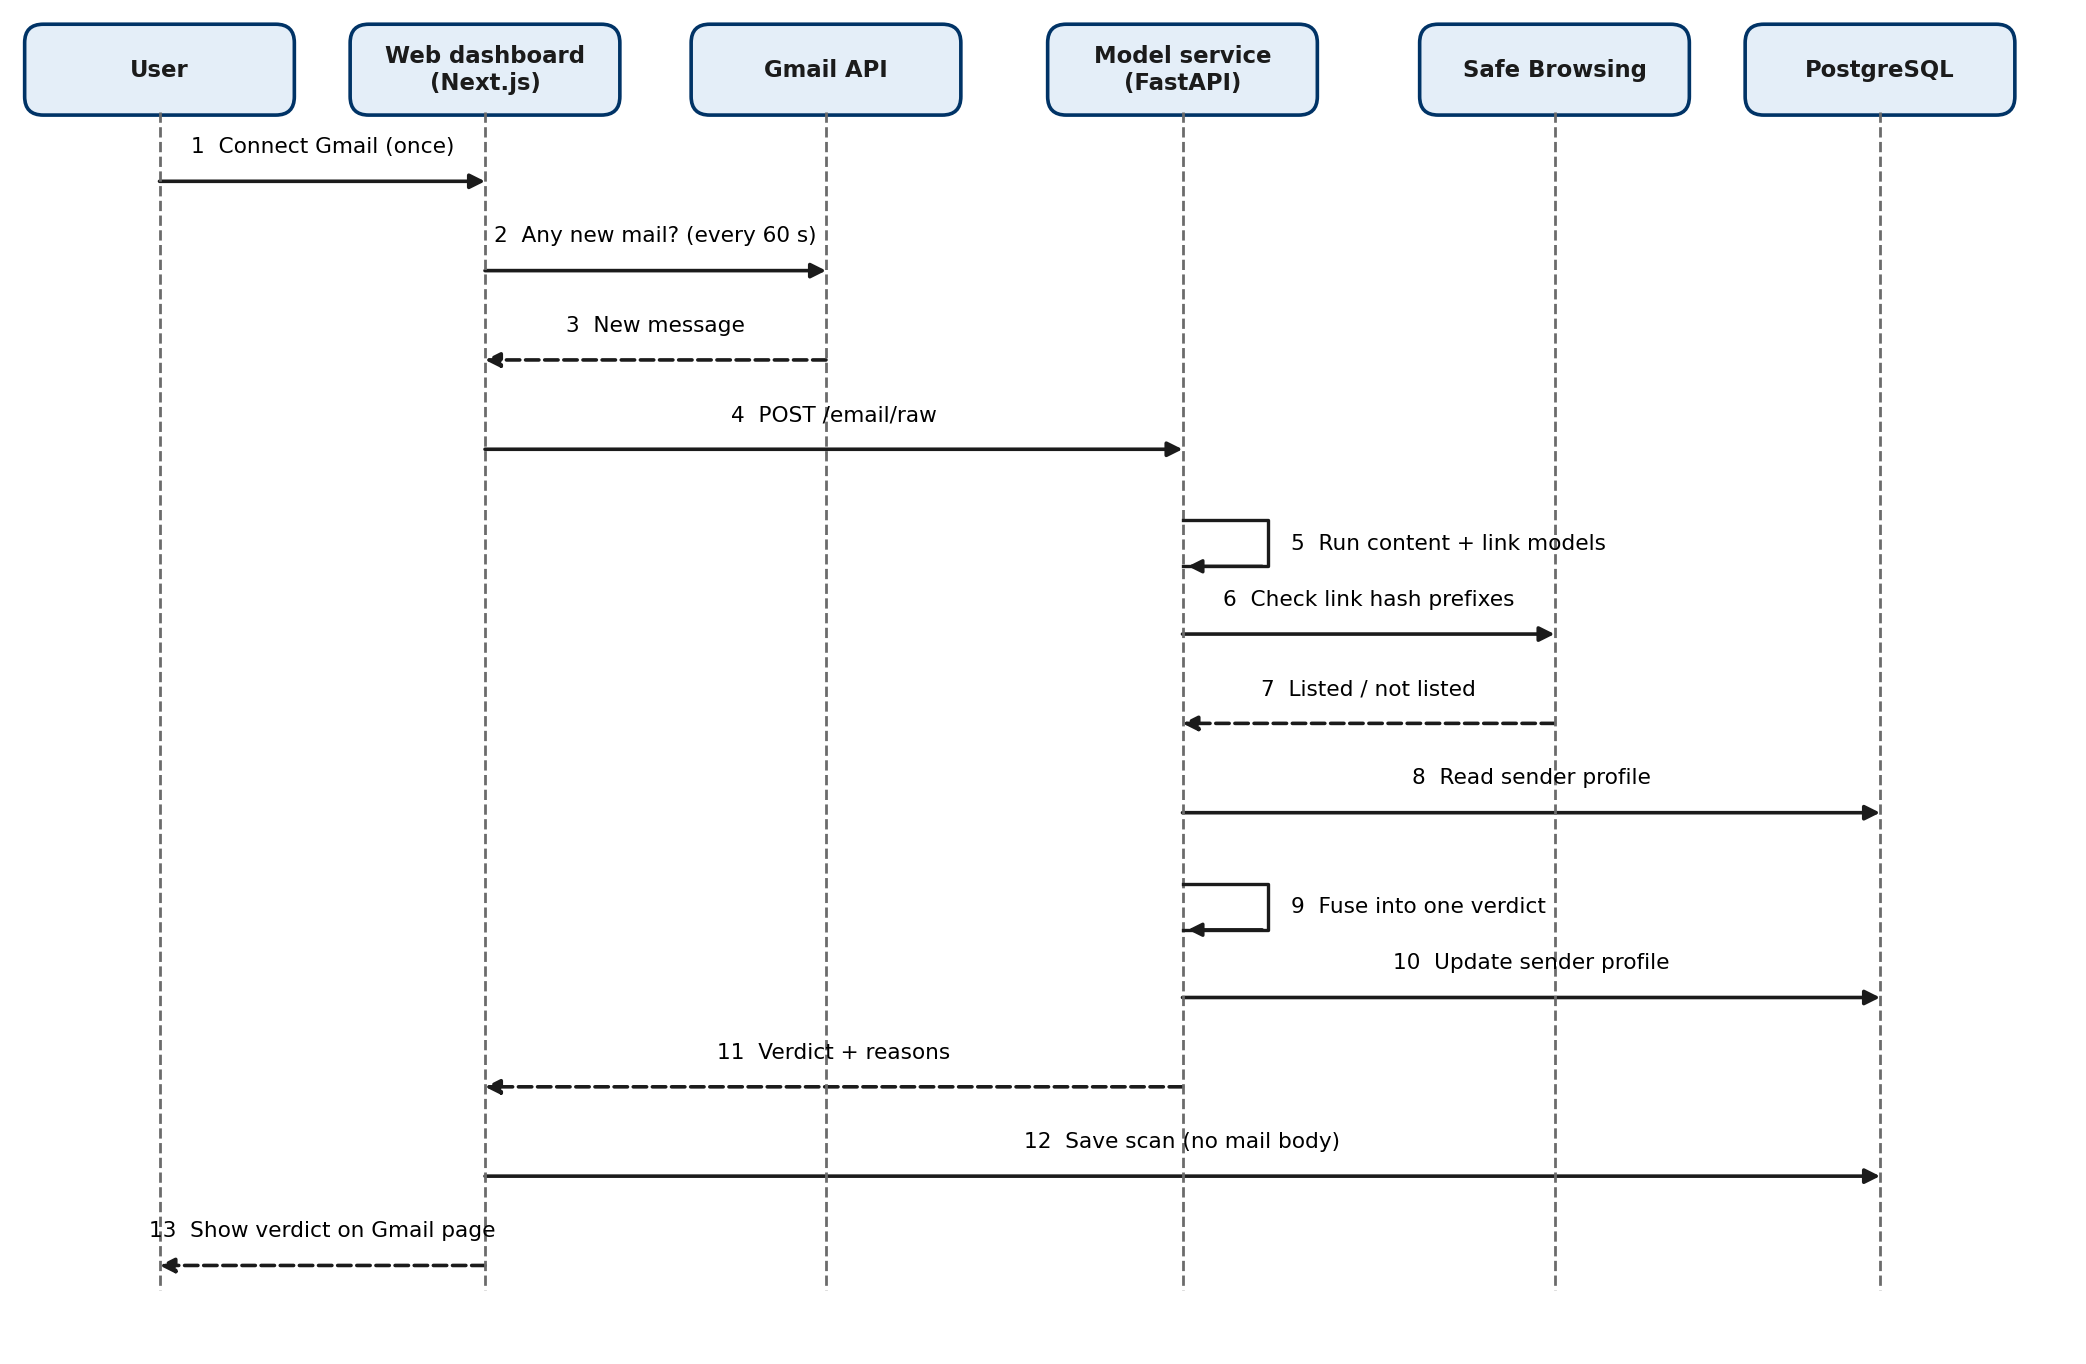
\includegraphics[width=\textwidth]{Chapter4/figures/sequence.png}
\caption{Sequence diagram for a Gmail message}
\label{fig:seq}
\end{figure}

\section{Summary}
This chapter presented the architecture, the modules of the three programs, the security measures, the database and five diagrams. The next chapter explains the algorithms in each part of the pipeline.

%--------------------------------------------------------------------------------------
}
